%% -*- mode: latex; -*-

\section{Spamassassin, Antivirus und Email via Perl}

An example article for the proceedings paper.

This article is written in ``dual language free style''\texttrademark,
sometimes additional subsections, sometimes just additional english
paragraphs, sometimes obvious examples are not translated. Please
report any language problems, you could imagine.

\subsection*{Autor}
Stefan Hornburg (Racke) \verb/<racke@linuxia.de>/

\subsection*{Bio Stefan Hornburg}

Dieser Abschnitt enth�lt eine Kurzbiographie (Bio). Beschreibe Dich
kurz in eigenen Worten und dem Stil Deiner Wahl.

This section contains your short biography. Describe yourself with
your own words and with your preferred style.

\subsection*{Abstract}
Die Bedeutung von Email f�r die Kommunikation hat einen hohen
Stellenwert erreicht und ist oftmals nicht aus dem t�glichen
Leben und aus der Arbeitswelt wegzudenken. Attacken auf dieses
wichtige Instrument mittlels SPAM, Viren und Phishing nehmen
kontinuierlich zu. N�tzliche Emails drohen in einer Flut von unerw�nschter
und potentiell sch�dlichen Post unterzugehen, wenn Gegenma�nahmen
nicht oder nur unzureichend greifen.

F�r Perl sind eine Reihe von Modulen vorhanden, die die Erstellung
von Programmen zum Zugriff auf Email und die Bewertung der Email
erleichtern:

	Net::SMTP (Emailversand)
	Mail::IMAPClient (Zugriff auf Email mit IMAP)
	Mail::Spamassassin (Spamassassin)
	ClamAV::Client (Clam Antivirus)
	
Nach einer kurzen Einf�hrung in die Benutzung dieser Module besch�ftigt
sich der Hauptteil des Vortrags mit der Beschreibung von Anwendungen
zur Verbesserung der Abwehr von SPAM, Viren und Phishing.

Zur Demonstration werden Emails von einem IMAP-Server heruntergeladen 
und von ClamAV auf Viren und Phishing gepr�ft und anschlie�end durch
SpamAssassin bewertet. Anschlie�end wird gezeigt, wie diese Emails vom
Server gel�scht oder in bestimmte Verzeichnisse auf dem IMAP-Server verschoben
werden k�nnen. Die Behandlung von Fehlerkennungen (False Positives)
wird ebenso erl�utert.

Im Anschlu� wird die Erstellung von Statistiken �ber das Aufkommen
von Viren und SPAM besprochen und wie man daraus Schl�sse zur Optimierung
zur Abwehr treffen kann.

\subsection{Mailversand mit Net::SMTP}
\begin{verbatim}
use Net::SMTP;

my $smtp = new Net::SMTP;
\end{verbatim}

\subsection{Virenscanner mit ClamAV::Client}

\subsection{Spamfilter mit Mail::Spamassassin}

\subsection{Mailempfang mit Mail::IMAPClient}

Eine IMAP-Verbindung kann einfach durch die Erzeugung eines
\verb/Mail::IMAPClient/-Objektes
mit den geeigneten Parametern hergestellt werden. Dafuer muessen
zumindestens der Servername (Server), Benutzername (User) und Passwort
(Password) uebergeben werden. Dann erfolgt der Verbindungsaufbau und die
Anmeldung automatisch.

\begin{verbatim}
use Mail::IMAPClient;

my $params = (Server => $server,
              User => $login,
              Password => $password);

my $client = new Mail::IMAPClient (%params);
\end{verbatim}

Dies ist nicht moeglich, wenn man eine SSL-geschuetzte Verbindung aufbauen
moechte. In diesem Fall erzeugt man die Verbindung mit dem
\verb/IO::Socket::SSL/-Modul: 

\WSIndex{IO::Socket::SSL}

\begin{verbatim}
use IO::Socket::SSL;
use Mail::IMAPClient;

my $conn;

unless ($conn = new IO::Socket::SSL->new ("${server}:imaps")) {
    die "$0: imaps connection to $server failed: $!\n";
}

$imap = new Mail::IMAPClient (Socket => $conn,
							  User => $user,
							  Password => $password);
\end{verbatim}

\subsection{Index, Fu�noten / Index, footnotes}
Im folgenden Abschnitt (nach der englischen �bersetzung) sind viele
W�rter f�r den Index markiert. Bitte hierf�r das Makro
\begin{verbatim}
 \WSIndex{indexwort}
\end{verbatim}
verwenden (siehe Quelltext). Die markierten W�rter werden im Index am
Ende des Dokumentes aufgelistet.

~

In the following paragraph many words are marked for the index. Please
use the macro
\begin{verbatim}
 \WSIndex{indexword}
\end{verbatim}
for marking (see source code). The marked words are listed in the index
at the end of the document.

\begin{quotation}
\noindent
Der \WSIndex{Scheik} von \WSIndex{Alessandria}\footnote{Auszug aus dem
\WSIndex{Wilhelm Hauff}-M�rchen / extraction from a fairy-tale of Wilhelm
Hauff. {\em Der Scheik von Alessandria},~\cite{racke:hauff}},
\WSIndex{Ali Banu}, war ein sonderbarer \WSIndex{Mann}; wenn er
morgens durch die Stra�en der Stadt ging, angetan mit einem
\WSIndex{Turban}, aus den \WSIndex{k�stlich}sten \WSIndex{Kaschmir}s
gewunden, mit dem \WSIndex{Festkleide} und dem reichen
\WSIndex{G�rtel}, der \WSIndex{f�nfzig} \WSIndex{Kamele} wert war,
wenn er einherging langsamen, gravit�tischen Schrittes, seine
\WSIndex{Stirn}e in finstere Falten gelegt, seine
\WSIndex{Augenbrauen} zusammengezogen, die \WSIndex{Augen}
niedergeschlagen und alle f�nf Schritte \WSIndex{gedankenvoll} seinen
langen, schwarzen Bart streichend; wenn er so hinging nach der
\WSIndex{Moschee}, um, wie es seine \WSIndex{W�rde} forderte, den
\WSIndex{Gl�ubige}n \WSIndex{Vorlesungen} �ber den \WSIndex{Koran} zu
halten: da blieben die Leute auf der Stra�e stehen, schauten ihm nach
und sprachen zueinander: ``Es ist doch ein sch�ner, stattlicher Mann,
und reich, ein reicher \WSIndex{Herr}'', setzte wohl ein anderer
hinzu, ``sehr reich; hat er nicht ein \WSIndex{Schlo�} am
\WSIndex{Hafen von Stambul}?  Hat er nicht \WSIndex{G�ter} und
\WSIndex{Felder} und viele tausend St�ck \WSIndex{Vieh} und viele
\WSIndex{Sklaven}?''

\end{quotation}

\subsection{Tabellen / Tables}

\subsubsection{tabularx}

\begin{table}[h]
\begin{tabularx}{\textwidth}{|p{3cm}|r|l|X|} \hline
Column A  & right-aligned  &
left-aligned & Restlicher Platz/remaining space  \\\hline

Perl    & 1.0  &  2.1  &  3.2  \\ \hline
Python  & 4    &  5    &  6    \\ \hline
Ruby    & 7    &  8    &  9    \\ \hline

\end{tabularx}
\caption{tabularx}
\end{table}

\subsubsection{\WSIndex{tabularx} mit multirow / tabularx with multirow}

\begin{table}[h]
\begin{tabularx}{\textwidth}{|p{3cm}|X|X|X|} \hline
Column A  & Column B  & Column C & Column D  \\\hline

\multirow{3}{5cm}{Gerade \newline Woche} & 1 & 2 & 3  \\ \cline{2-4}
                                         & 4 & 5 & 6  \\ \cline{2-4}
                                         & 7 & 8 & 9  \\ \hline
\end{tabularx}
\caption{tabularx mit multirow}
\end{table}

\subsubsection{tabularx mit multirow, ohne Trennlinien / tabularx with multirow, without separators}

\begin{center}
\begin{table}[h]
\begin{tabularx}{\textwidth}{p{3cm}XXX}
Spalte A  & Spalte B  & Spalte C & Spalte D  \\\hline

\multirow{3}{5cm}{Gerade \newline Woche} & 1 & 2 & 3  \\ 
                                         & 4 & 5 & 6  \\ 
                                         & 7 & 8 & 9  \\ 
\end{tabularx}
\caption{tabularx mit multirow ohne Trennlinien}
\end{table}
\end{center}

\subsubsection{supertabular*}
Beispiel f�r eine beeindruckend \WSIndex{unspektakul�re
Zahlenkolonne}.

Example for an impressively unspectacular column of figures.

\begin{center}
\bottomcaption{Die supertabular-Umgebung}
\begin{supertabular*}
 {\textwidth}{@{}p{40mm}p{40mm}p{70mm}@{}}
 040002 & 45221110 & ~   \\
 040002 & 45221120 & ~   \\
 040002 & 45221160 & (!) \\
 040002 & 23221110 & ~   \\
 040003 & 45221110 & ~   \\
 040003 & 45221120 & ~   \\
 usw.   & ~        & ~   \\
\end{supertabular*}
\end{center}

\subsection{verbatim}
Die bekannte Zahlenkolonne in verbatim:

The well-know column of figures with verbatim:

\begin{verbatim}
 040002 45221110
 040002 45221120
 040002 45221160        (!)
 040002 23221110
 040003 45221110
 040003 45221120
 usw.
\end{verbatim}


\subsection{figure, ref, cite}
Wie man Bilder einbindet wurde im Kapitel \ref{racke:section:graphics}
gezeigt. Hier verweisen wir nun auf eine ``irgendwo'' automatisch
platzierte Abbildung \ref{racke:fig:datenfluss}. Weiterhin verweisen wir
auf einen Eintrag in unserer Bibliographie, und zwar auf
\cite{racke:ExampleManual}.

Chapter \ref{racke:section:graphics} already showed how to include
images. Now we reference to a figure
\ref{racke:fig:datenfluss}, which is automatically placed ``anywhere''
by latex. Additionally we refer to an entry in the bibliography,
namely
\cite{racke:ExampleManual}.
\begin{figure}
 \centering
 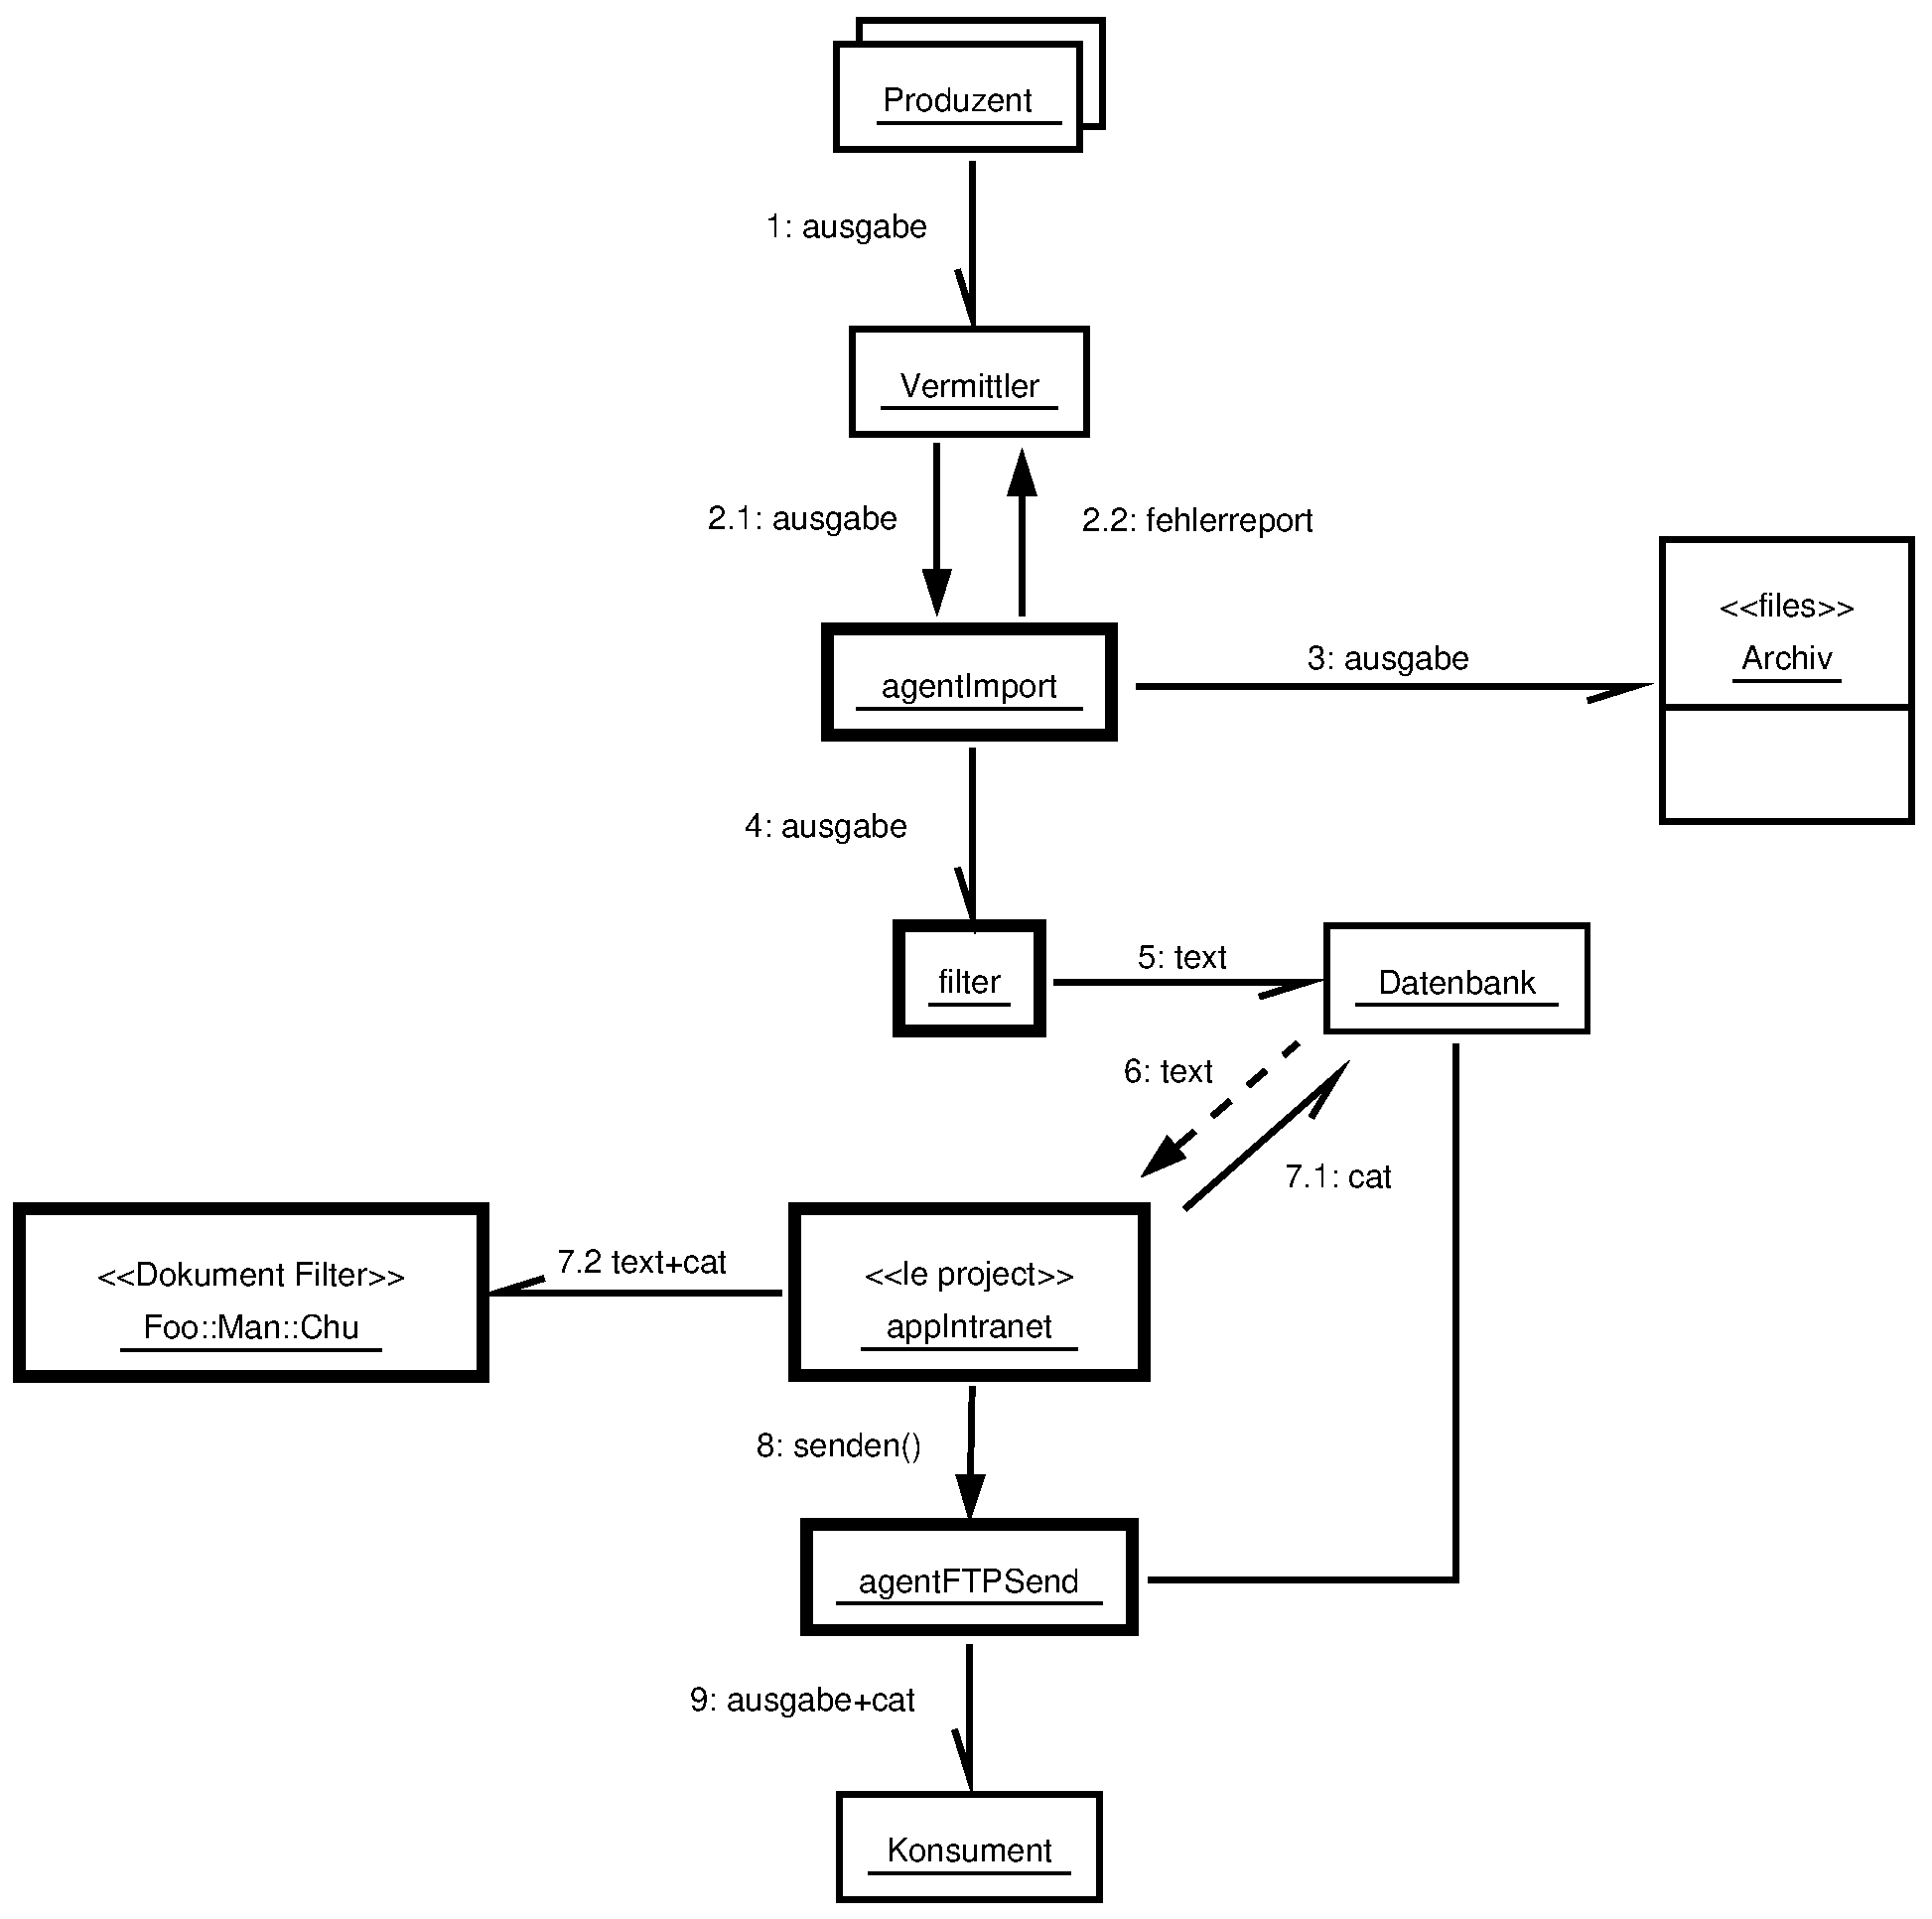
\includegraphics[width=\textwidth]{racke/datenfluss.eps}  % scale to textwidth
 \caption{Datenflu�}
 \label{racke:fig:datenfluss}
\end{figure}

\subsection{enumerate}
\begin{enumerate}
 \item Perl
   \begin{enumerate}
     \item strict
     \item warnings
     \item diagnostics
   \end{enumerate}
 \item Python
 \item Ruby
\end{enumerate}

\subsection{Verbatim Sourcecode}
\verbatiminput{racke/Categorization.pm}

\subsection{Listings}
\lstset{language=Perl,basicstyle=\footnotesize,columns=fixed}
\lstinputlisting{racke/Categorization.pm}

\begin{thebibliography}{99}

\bibitem{racke:hauff} Wilhelm Hauff. \emph{M�rchen-Almanach auf das Jahr
1827}. Project Gutenberg, 2003. \texttt{http://gutenberg.net}. 

\bibitem{racke:gnu} Free Software Foundation.
\emph{GNU's not Unix.} \texttt{http://www.gnu.org} 

\bibitem{racke:ExampleManual} Sabine Mustermann. \emph{The Example Manual -
Doing by Learning.} Addison-Snipes, Writing, Massachusetts, 1991.

\bibitem{racke:gnus} D. E. Knudson.
\emph{1966 World Gnus Almanac.} 

\bibitem{racke:Zomtec} Charles Zomtec, Inc.
\emph{Zomtec.} Green Bottle, Oregon, 2001.

\bibitem{racke:perlws} German Perl Workshop.
\emph{German Perl Workshop Website.}
\texttt{http://www.perl-workshop.de}

\end{thebibliography}

